\documentclass[12pt,a4paper]{report}

% ============================================================================
% PACKAGES
% ============================================================================
\usepackage[utf8]{inputenc}
\usepackage[T1]{fontenc}
\usepackage{lmodern}
\usepackage[margin=1in]{geometry}
\usepackage{graphicx}
\usepackage{xcolor}
\usepackage{hyperref}
\usepackage{tikz}
\usepackage{longtable}
\usepackage{booktabs}
\usepackage{fancyhdr}
\usepackage{titlesec}
\usepackage{listings}
\usepackage{enumitem}

% TikZ Libraries
\usetikzlibrary{shapes.geometric, arrows.meta, positioning, fit, backgrounds}

% ============================================================================
% COLORS
% ============================================================================
\definecolor{primaryblue}{RGB}{26, 54, 93}
\definecolor{secondaryblue}{RGB}{59, 130, 246}
\definecolor{accentgreen}{RGB}{34, 197, 94}
\definecolor{warningorange}{RGB}{249, 115, 22}
\definecolor{dangerred}{RGB}{239, 68, 68}
\definecolor{lightgray}{RGB}{243, 244, 246}
\definecolor{darkgray}{RGB}{75, 85, 99}
\definecolor{staffpurple}{RGB}{168, 85, 247}

% ============================================================================
% HYPERREF SETUP
% ============================================================================
\hypersetup{
    colorlinks=true,
    linkcolor=primaryblue,
    urlcolor=secondaryblue,
    pdftitle={EduX - Staff Management Guide},
    pdfauthor={EduX Development Team},
}

% ============================================================================
% HEADER/FOOTER
% ============================================================================
\pagestyle{fancy}
\fancyhf{}
\fancyhead[L]{\textcolor{darkgray}{\small EduX School Management System}}
\fancyhead[R]{\textcolor{darkgray}{\small Staff Management Guide}}
\fancyfoot[C]{\textcolor{darkgray}{\thepage}}
\renewcommand{\headrulewidth}{0.4pt}

% ============================================================================
% TITLE FORMATTING
% ============================================================================
\titleformat{\chapter}[display]
  {\normalfont\huge\bfseries\color{primaryblue}}
  {\chaptertitlename\ \thechapter}{20pt}{\Huge}

\titleformat{\section}
  {\normalfont\Large\bfseries\color{primaryblue}}
  {\thesection}{1em}{}

\titleformat{\subsection}
  {\normalfont\large\bfseries\color{secondaryblue}}
  {\thesubsection}{1em}{}

% ============================================================================
% DOCUMENT
% ============================================================================
\begin{document}

% ----------------------------------------------------------------------------
% TITLE PAGE
% ----------------------------------------------------------------------------
\begin{titlepage}
    \centering
    \vspace*{2cm}
    
    {\Huge\bfseries\textcolor{primaryblue}{EduX}\par}
    \vspace{0.5cm}
    {\Large\textcolor{secondaryblue}{School Management System}\par}
    
    \vspace{2cm}
    
    
\begin{tikzpicture}
        \node[draw=primaryblue, line width=2pt, rounded corners=10pt, 
              minimum width=8cm, minimum height=3cm, fill=lightgray] 
              {\Huge\bfseries\textcolor{primaryblue}{Staff Management}};
    \end{tikzpicture}
    
    \vfill
    
    {\large\textcolor{darkgray}{Version 1.0}\par}
    {\large\textcolor{darkgray}{\today}\par}
\end{titlepage}

\tableofcontents
\newpage

% ============================================================================
% CHAPTER 1: OVERVIEW
% ============================================================================
\chapter{Staff Management Overview}

\section{Introduction}

The Staff Management module handles all aspects of employee administration including profiles, attendance, leave management, subject assignments, and payroll.

\section{Staff Module Components}

\begin{center}
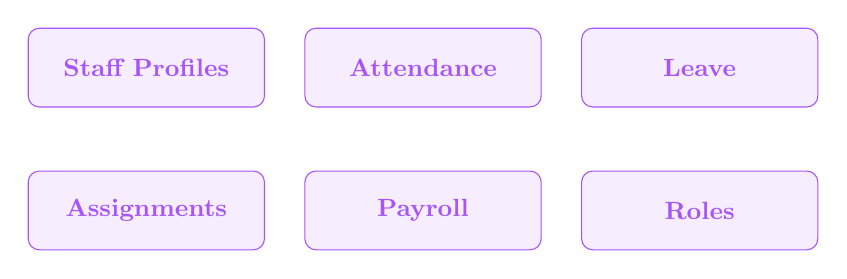
\begin{tikzpicture}[
    node distance=1cm,
    comp/.style={draw=staffpurple, rounded corners, minimum width=3cm, 
                 minimum height=1cm, fill=staffpurple!10, align=center, 
                 font=\small\bfseries, text=staffpurple}
]
    \node[comp] (profiles) at (0,0) {Staff Profiles};
    \node[comp, right=0.5cm of profiles] (attendance) {Attendance};
    \node[comp, right=0.5cm of attendance] (leave) {Leave};
    \node[comp, below=0.8cm of profiles] (assignments) {Assignments};
    \node[comp, right=0.5cm of assignments] (payroll) {Payroll};
    \node[comp, right=0.5cm of payroll] (roles) {Roles};
\end{tikzpicture}
\end{center}

\section{Staff Roles}

\begin{center}
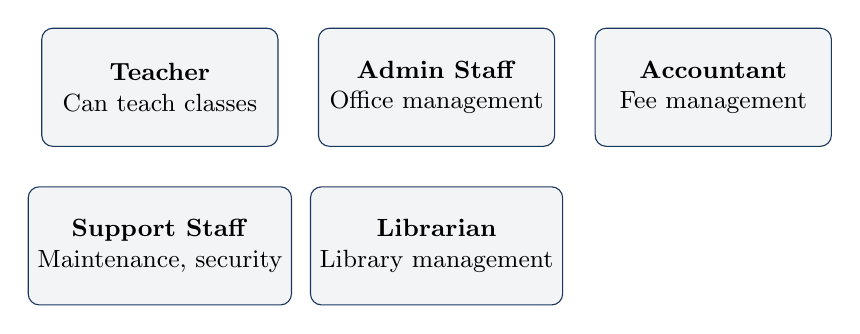
\begin{tikzpicture}[
    role/.style={draw=primaryblue, rounded corners, minimum width=3cm, 
                 minimum height=1.5cm, fill=lightgray, align=center, font=\small}
]
    \node[role] (teacher) at (0,0) {\textbf{Teacher}\\Can teach classes};
    \node[role, right=0.5cm of teacher] (admin) {\textbf{Admin Staff}\\Office management};
    \node[role, right=0.5cm of admin] (accountant) {\textbf{Accountant}\\Fee management};
    \node[role, below=0.5cm of teacher] (support) {\textbf{Support Staff}\\Maintenance, security};
    \node[role, below=0.5cm of admin] (librarian) {\textbf{Librarian}\\Library management};
\end{tikzpicture}
\end{center}

% ============================================================================
% CHAPTER 2: STAFF PROFILES
% ============================================================================
\chapter{Staff Profiles}

\section{Adding Staff Members}

Navigate to \texttt{Staff} $\rightarrow$ \texttt{Add Staff}

\subsection{Personal Information}

\begin{longtable}{@{}p{4cm}p{3cm}p{6cm}@{}}
\toprule
\textbf{Field} & \textbf{Required} & \textbf{Description} \\
\midrule
\endhead
Employee ID & Yes & Unique identifier \\
First Name & Yes & Staff first name \\
Last Name & Yes & Staff last name \\
Date of Birth & No & Birth date \\
Gender & Yes & Male / Female \\
CNIC & No & National ID number \\
Phone & Yes & Primary contact \\
Alternate Phone & No & Secondary contact \\
Email & No & Email address \\
Address & No & Residential address \\
City & No & City of residence \\
\bottomrule
\end{longtable}

\subsection{Professional Information}

\begin{longtable}{@{}p{4cm}p{3cm}p{6cm}@{}}
\toprule
\textbf{Field} & \textbf{Required} & \textbf{Description} \\
\midrule
\endhead
Role & Yes & Staff role (Teacher, etc.) \\
Designation & Yes & Job title \\
Department & No & Academic / Admin \\
Qualification & No & Highest degree \\
Specialization & No & Subject expertise \\
Experience Years & No & Prior experience \\
Previous Employer & No & Last workplace \\
Joining Date & Yes & Date of joining \\
\bottomrule
\end{longtable}

\subsection{Financial Information}

\begin{longtable}{@{}p{4cm}p{3cm}p{6cm}@{}}
\toprule
\textbf{Field} & \textbf{Required} & \textbf{Description} \\
\midrule
\endhead
Basic Salary & Yes & Monthly basic salary \\
Bank Name & No & Salary bank \\
Account Number & No & Bank account number \\
\bottomrule
\end{longtable}

\section{Staff Status}

\begin{center}

\begin{tikzpicture}[
    status/.style={draw=#1, rounded corners, minimum width=2.2cm, 
                   minimum height=0.8cm, fill=#1!15, font=\small\bfseries, text=#1}
]
    \node[status=accentgreen] (active) at (0,0) {Active};
    \node[status=secondaryblue, right=0.3cm of active] (leave) {On Leave};
    \node[status=warningorange, right=0.3cm of leave] (resigned) {Resigned};
    \node[status=dangerred, right=0.3cm of resigned] (terminated) {Terminated};
\end{tikzpicture}
\end{center}

% ============================================================================
% CHAPTER 3: STAFF ATTENDANCE
% ============================================================================
\chapter{Staff Attendance}

\section{Marking Attendance}

Navigate to \texttt{Staff} $\rightarrow$ \texttt{Attendance}

\begin{enumerate}[leftmargin=*]
    \item Select date
    \item View staff list
    \item Mark status for each staff
    \item Enter check-in/check-out times
    \item Add remarks if needed
    \item Save attendance
\end{enumerate}

\section{Attendance Statuses}

\begin{center}

\begin{tikzpicture}[
    status/.style={draw=#1, rounded corners, minimum width=2cm, 
                   minimum height=0.8cm, fill=#1!15, font=\small\bfseries, text=#1}
]
    \node[status=accentgreen] (present) at (0,0) {Present};
    \node[status=dangerred, right=0.3cm of present] (absent) {Absent};
    \node[status=warningorange, right=0.3cm of absent] (late) {Late};
    \node[status=secondaryblue, right=0.3cm of late] (leave) {Leave};
    \node[status=staffpurple, right=0.3cm of leave] (half) {Half Day};
\end{tikzpicture}
\end{center}

\section{Check-in / Check-out}

Staff attendance includes timing:
\begin{itemize}[leftmargin=*]
    \item \textbf{Check-in Time} -- Arrival time
    \item \textbf{Check-out Time} -- Departure time
    \item Automatic late detection based on school timing
\end{itemize}

% ============================================================================
% CHAPTER 4: LEAVE MANAGEMENT
% ============================================================================
\chapter{Leave Management}

\section{Leave Types}

\begin{center}
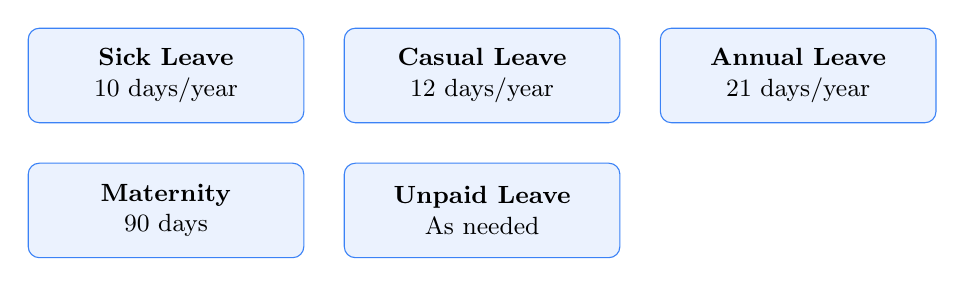
\begin{tikzpicture}[
    leave/.style={draw=secondaryblue, rounded corners, minimum width=3.5cm, 
                  minimum height=1.2cm, fill=secondaryblue!10, align=center, 
                  font=\small}
]
    \node[leave] (sick) at (0,0) {\textbf{Sick Leave}\\10 days/year};
    \node[leave, right=0.5cm of sick] (casual) {\textbf{Casual Leave}\\12 days/year};
    \node[leave, right=0.5cm of casual] (annual) {\textbf{Annual Leave}\\21 days/year};
    \node[leave, below=0.5cm of sick] (maternity) {\textbf{Maternity}\\90 days};
    \node[leave, below=0.5cm of casual] (unpaid) {\textbf{Unpaid Leave}\\As needed};
\end{tikzpicture}
\end{center}

\section{Leave Request Flow}

\begin{center}
\begin{tikzpicture}[
    node distance=1cm,
    step/.style={draw=primaryblue, rounded corners, minimum width=3.5cm, 
                 minimum height=0.9cm, fill=lightgray, align=center, font=\small},
    arrow/.style={-{Stealth}, thick, secondaryblue}
]
    \node[step] (submit) {Staff Submits Request};
    \node[step, below=of submit] (pending) {Pending Approval};
    \node[step, below left=1cm and -0.5cm of pending] (approved) {Approved};
    \node[step, below right=1cm and -0.5cm of pending] (rejected) {Rejected};
    \node[step, below=of approved] (marked) {Attendance Marked};
    
    \draw[arrow] (submit) -- (pending);
    \draw[arrow] (pending) -- node[left, font=\scriptsize] {approve} (approved);
    \draw[arrow] (pending) -- node[right, font=\scriptsize] {reject} (rejected);
    \draw[arrow] (approved) -- (marked);
\end{tikzpicture}
\end{center}

\section{Creating Leave Request}

\begin{enumerate}[leftmargin=*]
    \item Go to \texttt{Staff} $\rightarrow$ \texttt{Leave} $\rightarrow$ \texttt{New Request}
    \item Select staff member
    \item Choose leave type
    \item Set start and end dates
    \item Enter reason
    \item Submit request
\end{enumerate}

\section{Approving Leave Requests}

Administrators can:
\begin{enumerate}[leftmargin=*]
    \item View pending requests
    \item Check leave balance
    \item Approve or reject with remarks
    \item View leave calendar
\end{enumerate}

% ============================================================================
% CHAPTER 5: SUBJECT ASSIGNMENTS
% ============================================================================
\chapter{Subject Assignments}

\section{Overview}

Assign teachers to classes and subjects for the academic year.

\section{Creating Assignments}

Navigate to \texttt{Staff} $\rightarrow$ \texttt{Assignments}

\begin{longtable}{@{}p{4cm}p{3cm}p{6cm}@{}}
\toprule
\textbf{Field} & \textbf{Required} & \textbf{Description} \\
\midrule
\endhead
Staff Member & Yes & Select teacher \\
Class & Yes & Assigned class \\
Section & No & Specific section or all \\
Subject & Yes & Subject to teach \\
Academic Year & Yes & Current year \\
Is Class Teacher & No & Primary class responsibility \\
\bottomrule
\end{longtable}

\section{Assignment Matrix}

\begin{center}
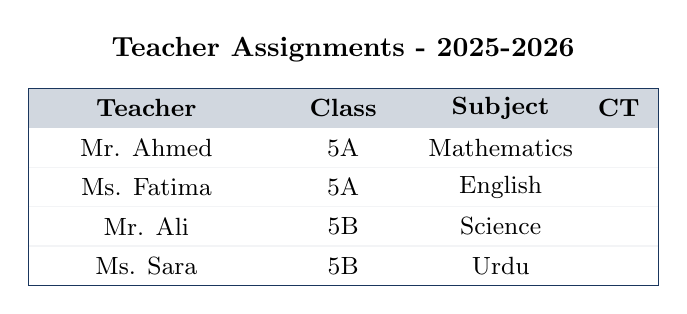
\begin{tikzpicture}
    % Title
    \node[font=\bfseries] at (4,3) {Teacher Assignments - 2025-2026};
    
    % Headers
    \fill[primaryblue!20] (0,2) rectangle (8,2.5);
    \node[font=\small\bfseries] at (1.5,2.25) {Teacher};
    \node[font=\small\bfseries] at (4,2.25) {Class};
    \node[font=\small\bfseries] at (6,2.25) {Subject};
    \node[font=\small\bfseries] at (7.5,2.25) {CT};
    
    % Rows
    \foreach \y/\teacher/\class/\subject/\ct in {
        1.5/Mr. Ahmed/5A/Mathematics/\checkmark,
        1/Ms. Fatima/5A/English/,
        0.5/Mr. Ali/5B/Science/\checkmark,
        0/Ms. Sara/5B/Urdu/
    } {
        \draw[lightgray] (0,\y) -- (8,\y);
        \node[font=\small] at (1.5,\y+0.25) {\teacher};
        \node[font=\small] at (4,\y+0.25) {\class};
        \node[font=\small] at (6,\y+0.25) {\subject};
        \node[font=\small] at (7.5,\y+0.25) {\ct};
    }
    
    \draw[primaryblue] (0,0) rectangle (8,2.5);
\end{tikzpicture}
\end{center}

% ============================================================================
% CHAPTER 6: PAYROLL
% ============================================================================
\chapter{Payroll Management}

\section{Payroll Overview}

Monthly salary processing including:
\begin{itemize}[leftmargin=*]
    \item Basic salary
    \item Allowances
    \item Deductions
    \item Attendance-based calculations
\end{itemize}

\section{Salary Components}

\begin{center}
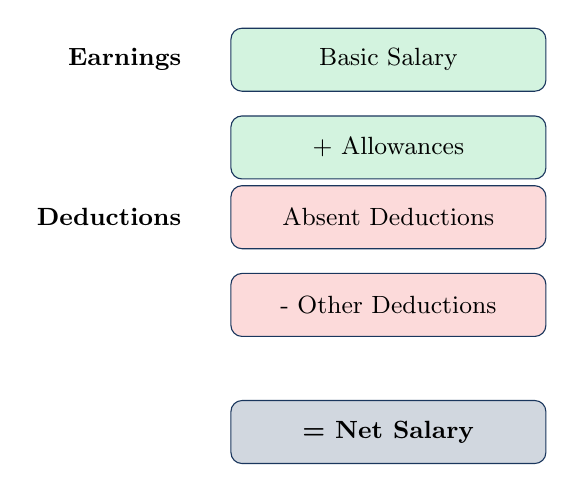
\begin{tikzpicture}[
    node distance=0.8cm,
    comp/.style={draw=primaryblue, rounded corners, minimum width=4cm, 
                 minimum height=0.8cm, fill=lightgray, align=center, font=\small}
]
    % Earnings
    \node[comp, fill=accentgreen!20] (basic) at (0,2) {Basic Salary};
    \node[comp, fill=accentgreen!20, below=0.3cm of basic] (allow) {+ Allowances};
    \node[font=\small\bfseries, left=0.5cm of basic] {Earnings};
    
    % Deductions
    \node[comp, fill=dangerred!20] (absent) at (0,0) {Absent Deductions};
    \node[comp, fill=dangerred!20, below=0.3cm of absent] (other) {- Other Deductions};
    \node[font=\small\bfseries, left=0.5cm of absent] {Deductions};
    
    % Net
    \node[comp, fill=primaryblue!20, below=0.8cm of other] (net) {\textbf{= Net Salary}};
\end{tikzpicture}
\end{center}

\section{Generating Payroll}

\begin{enumerate}[leftmargin=*]
    \item Go to \texttt{Staff} $\rightarrow$ \texttt{Payroll}
    \item Select month
    \item Click \texttt{Generate Payroll}
    \item System calculates:
    \begin{itemize}
        \item Working days in month
        \item Days present/absent
        \item Leave days (paid/unpaid)
        \item Allowances and deductions
    \end{itemize}
    \item Review calculations
    \item Confirm payroll
\end{enumerate}

\section{Salary Slip}

\begin{center}
\begin{tikzpicture}[
    box/.style={draw=primaryblue, minimum width=7cm, align=left, font=\small, 
                fill=lightgray, rounded corners}
]
    \node[box, minimum height=5.5cm] at (0,0) {
        \centering\textbf{SALARY SLIP}\\
        \textit{January 2025}\\[0.2cm]
        \rule{6.5cm}{0.4pt}\\[0.1cm]
        \textbf{Employee:} Mr. Ahmed Khan\\
        \textbf{Designation:} Senior Teacher\\
        \textbf{Department:} Academic\\[0.1cm]
        \rule{6.5cm}{0.4pt}\\[0.1cm]
        \textbf{Earnings:}\\
        Basic Salary \hfill PKR 50,000\\
        Transport Allowance \hfill PKR 5,000\\[0.1cm]
        \textbf{Deductions:}\\
        Absent (2 days) \hfill PKR 3,333\\[0.1cm]
        \rule{6.5cm}{0.4pt}\\[0.1cm]
        \textbf{Net Salary} \hfill \textbf{PKR 51,667}\\[0.2cm]
        \rule{3cm}{0.4pt}\\
        Authorized Signature
    };
\end{tikzpicture}
\end{center}

\section{Payment Processing}

\begin{enumerate}[leftmargin=*]
    \item Select staff members to pay
    \item Choose payment mode (Cash / Bank Transfer / Cheque)
    \item Enter reference details
    \item Mark as paid
    \item Print salary slips
\end{enumerate}

% ============================================================================
% CHAPTER 7: REPORTS
% ============================================================================
\chapter{Staff Reports}

\section{Available Reports}

\begin{longtable}{@{}p{4cm}p{9cm}@{}}
\toprule
\textbf{Report} & \textbf{Description} \\
\midrule
\endhead
Staff Directory & Complete staff list with details \\
Attendance Report & Monthly attendance summary \\
Leave Report & Leave taken by staff \\
Leave Balance & Remaining leave per type \\
Payroll Report & Salary details for period \\
Assignment Report & Teacher-class-subject mapping \\
\bottomrule
\end{longtable}

\section{Exporting Reports}

All reports can be exported as:
\begin{itemize}[leftmargin=*]
    \item \textbf{PDF} -- Formatted document
    \item \textbf{Excel} -- Raw data
\end{itemize}

\end{document}
